% !TeX program = xelatex
% =====================================================================
% 合肥工业大学《计算机图形学》课程设计报告模板
% 编译方式：使用 XeLaTeX 编译两次（保证目录页码正确）
%   命令行：xelatex 课程设计报告.tex
%          xelatex 课程设计报告.tex
%   推荐编辑器：TeXstudio / VSCode + LaTeX Workshop（设置默认编译器为 xelatex）
%   系统需安装 CTeX 套装、TeX Live 或 MiKTeX 完整版（含中文字体）
% =====================================================================

\documentclass[12pt, a4paper]{article}

% ---------- 宏包 ----------
\usepackage[UTF8, scheme=plain]{ctex}
\usepackage{geometry}
\usepackage{graphicx}
\usepackage{array}
\usepackage{tabularx}
\usepackage{multirow}
\usepackage{makecell}
\usepackage{titlesec}
\usepackage{fancyhdr}
\usepackage{setspace}
\usepackage{enumitem}
\usepackage{hyperref}
\usepackage{listings}
\usepackage{xcolor}
\usepackage{float}
\usepackage{caption}
\usepackage{indentfirst}
\usepackage{amsmath}
\usepackage{amssymb}  % 推荐也加上
% ---------- 页面 ----------
\geometry{a4paper, left=2.5cm, right=2.5cm, top=2.5cm, bottom=2.5cm}

% ---------- 章节标题 ----------
% 主章节用中文序号（一、二、三...），小节用 1.1, 1.2...
\renewcommand{\thesubsection}{\arabic{section}.\arabic{subsection}}
\titleformat{\section}
    {\centering\Large\bfseries}
    {\chinese{section}、}
    {0.3em}{}
\titleformat{\subsection}
    {\large\bfseries}
    {\thesubsection}
    {0.8em}{}
\titlespacing*{\section}{0pt}{1.2em}{0.8em}
\titlespacing*{\subsection}{0pt}{0.8em}{0.5em}

% ---------- 行距与缩进 ----------
\linespread{1.5}
\setlength{\parindent}{2em}

% ---------- 超链接 ----------
\hypersetup{
    colorlinks=true,
    linkcolor=black,
    urlcolor=blue,
    citecolor=black
}

% ---------- 代码样式 ----------
\definecolor{codegray}{rgb}{0.5,0.5,0.5}
\definecolor{codegreen}{rgb}{0.0,0.5,0.0}
\definecolor{codeblue}{rgb}{0.1,0.3,0.7}
\definecolor{codered}{rgb}{0.7,0.1,0.1}
\lstdefinestyle{mycode}{
    basicstyle=\ttfamily\small,
    breaklines=true,
    breakatwhitespace=false,
    frame=single,
    rulecolor=\color{black!30},
    numbers=left,
    numberstyle=\tiny\color{codegray},
    keywordstyle=\color{codeblue}\bfseries,
    commentstyle=\color{codegreen}\itshape,
    stringstyle=\color{codered},
    showstringspaces=false,
    tabsize=4,
    captionpos=b,
    columns=fullflexible,
    aboveskip=0.8em,
    belowskip=0.8em
}
\lstset{style=mycode}

\begin{document}

% =====================================================================
% 封面（附件二）
% =====================================================================
\thispagestyle{empty}


\vspace{2em}

\begin{center}
    {\fontsize{56pt}{72pt}\selectfont\heiti 合肥工业大学}

    \vspace{1.2em}

    {\fontsize{64pt}{80pt}\selectfont\heiti 课\hspace{0.3em}程\hspace{0.3em}设\hspace{0.3em}计}
\end{center}

\vspace{5em}

\begin{center}
    \zihao{3}
    \renewcommand{\arraystretch}{2.2}
    \begin{tabular}{rl}
        设\ 计\ 题\ 目 & \underline{\makebox[8cm]{计算机图形学课程设计}} \\
        学\ 生\ 姓\ 名 & \underline{\makebox[8cm]{张致远}} \\
        学\hspace{2.5em}号 & \underline{\makebox[8cm]{2023213980}} \\
        专\ 业\ 班\ 级 & \underline{\makebox[8cm]{信息与计算科学23-1班}} \\
        指\ 导\ 教\ 师 & \underline{\makebox[8cm]{霍星}} \\
    \end{tabular}
\end{center}

\vfill

\begin{center}
    {\zihao{3} \makebox[2cm]{2026} 年 \makebox[2cm]{5} 月 \makebox[2cm]{24} 日}
\end{center}

\vspace{2em}

\newpage

% =====================================================================
% 任务书（附件三）
% =====================================================================
\thispagestyle{empty}

\noindent
\hspace{2em}{\LARGE\bfseries 合肥工业大学课程设计任务书}

\vspace{1em}

\noindent
\renewcommand{\arraystretch}{1.4}
\begin{tabular}{|c|p{6cm}|c|p{4cm}|}
    \hline
    \makecell{设计\\题目} & 计算机图形学课程设计\hspace{0pt} & 成绩 & \hspace{0pt} \\
    \hline
    \makecell[t]{课\\程\\设\\计\\主\\要\\内\\容}
    & \multicolumn{3}{p{12cm}|}{
        \raggedright
        完成了所有四个题目，并用python+pygame库设计了交互式的UI来呈现题目一：星空绘制，题目二：鸭子，题目三：游泳的鸭子，题目四：松鼠松果，并在这个过程中总结了收获
        基本绘制直线，圆，填充等算法没有调包，均为基础手写完成。

        \vspace{11cm}
    } \\
    \hline
    \makecell[t]{指\\导\\教\\师\\评\\语}
    & \multicolumn{3}{p{12cm}|}{
        \raggedright
        {\footnotesize\textbf{建议：从学生的工作态度、工作量、设计（论文）的创造性、学术性、实用性及书面表达能力等方面给出评价。}}
        \vspace{5.5cm}

        \hfill 签名：\makebox[2.5cm]{} \hspace{1em} 2025 \makebox[1cm]{} 年 \makebox[1cm]{} 月 \makebox[1cm]{} 日
        \vspace{0.3em}
    } \\
    \hline
\end{tabular}

\newpage

% =====================================================================
% 目录
% =====================================================================
\thispagestyle{empty}

\begin{center}
    {\zihao{2}\bfseries 目\hspace{2em}录}
\end{center}

\vspace{1.5em}

{
\zihao{4}
\renewcommand{\baselinestretch}{1.8}\selectfont
\noindent
一、\ 设计题目与要求 \dotfill \pageref{sec:one}\\
\hspace*{2em}1.1\ \ 设计题目 \dotfill \\
\hspace*{2em}1.2\ \ 设计内容 \dotfill \\
\hspace*{2em}1.3\ \ 设计目标 \dotfill \\
二、\ 系统功能介绍 \dotfill \pageref{sec:two}\\
三、\ 方案设计 \dotfill \pageref{sec:three}\\
\hspace*{2em}3.1\ \ 总体方案设计 \dotfill \\
四、\ 详细设计 \dotfill \pageref{sec:four}\\
\hspace*{2em}4.1\ \ 题目一：星空图绘制 \dotfill \\
\hspace*{2em}4.2\ \ 题目二：鸭子绘制与变换 \dotfill \\
\hspace*{2em}4.3\ \ 题目三：游泳的鸭子 \dotfill \\
\hspace*{2em}4.4\ \ 题目四：松树与松果 \dotfill \\
五、\ 总结 \dotfill \pageref{sec:five}\\
\hspace*{2em}5.1\ \ 程序结构优缺点分析 \dotfill \\
\hspace*{2em}5.2\ \ 出错原因分析 \dotfill \\
}

\newpage

% =====================================================================
% 正文
% =====================================================================
\setcounter{page}{1}
\pagestyle{plain}

% --------- 一、设计题目与要求 ---------
\section{设计题目与要求}\label{sec:one}

\subsection{设计题目}

基于 Python 与 Pygame 的计算机图形学综合作品——星空图、鸭子动画与松树场景绘制系统。

\subsection{设计内容}

本作品按合肥工业大学《计算机图形学》课程设计任务书的要求，使用 Python 与 Pygame
实现以下四个子模块：
\begin{enumerate}[label=（\arabic*）, leftmargin=*]
    \item \textbf{题目一（必做）}\ 利用点、线、圆、多边形等计算机基本图元绘制一幅星空图；
    \item \textbf{题目二}\ 绘制一只鸭子，并对鸭子进行旋转、平移等几何变换；
    \item \textbf{题目三（提高题）}\ 绘制一只游泳的鸭子；
    \item \textbf{题目四（难题）}\ 绘制一棵枝叶摇动的松树和掉落的松果。
\end{enumerate}

本报告依次给出四个子模块的方案设计、详细设计与实现，其中题目一已完整实现，
其余子模块的实现随开发推进逐步补充。整套作品强调以下两点：
\begin{itemize}[leftmargin=*]
    \item \textbf{底层算法自实现}：直线、圆、多边形填充等基本图元的生成
    \textit{不}直接调用 Pygame 提供的高层 API（如 \texttt{pygame.draw.line}），
    而是亲自实现 Bresenham 直线生成、中点画圆、扫描线多边形填充等经典算法，
    通过 \texttt{Surface.set\_at()} 直接写像素，体现对图形学底层原理的掌握。
    \item \textbf{统一交互框架}：所有子模块共享同一套自定义 UI 组件（按钮、开关、滑块），
    具备菜单栏 / 工具栏 / 参数面板 / 主画布的统一布局，
    符合任务书"界面美观、衔接自然、注重交互性"的要求。
\end{itemize}

\subsection{设计目标}

\begin{enumerate}[label=（\arabic*）, leftmargin=*]
    \item 巩固和综合应用所学的计算机图形学理论知识，培养学生理论联系实际和独立思考问题的能力；
    \item 掌握 Bresenham 直线、中点画圆、扫描线多边形填充等基础图元生成算法的推导与编码实现；
    \item 培养图形应用软件的工程化开发能力——模块划分、控件封装、性能优化与文档撰写；
    \item 通过四道题目的递进设计，体会从\textit{静态图形} → \textit{几何变换} →
    \textit{动画} → \textit{复杂交互动画}的渐进过程，强化对二维图形系统的整体认识。
\end{enumerate}

% --------- 二、系统功能介绍 ---------
\section{系统功能介绍}\label{sec:two}

整套作品由四个独立子模块组成，每个子模块对应任务书中的一道题目，均以一个
独立可执行 Python 脚本形式提供。所有子模块共享统一的界面骨架：
\textbf{顶部工具栏} + \textbf{右侧参数控制面板} + \textbf{主画布}。

\subsubsection*{题目一：星空图绘制}
启动 \texttt{python 题目1\_星空图/main.py} 进入星空场景，主要功能包括：
\begin{itemize}[leftmargin=*]
    \item \textbf{场景渲染}：渐变天空背景；满天可调密度的小星星；
    一颗会缓慢自转、带光芒的大五角星；一轮带月坑与光晕的月亮；
    沿对角线划过的彗星；锯齿状的山脉剪影地平线。
    \item \textbf{工具栏按钮}：\textit{重新生成}（随机化星点与山脉）、
    \textit{切换主题}（深夜 / 黄昏 / 极光三套配色）、
    \textit{保存图片}（导出当前画布为 PNG）、\textit{关于}（弹窗显示算法说明）。
    \item \textbf{工具栏开关}：\textit{月亮 / 彗星 / 动画}的独立显示开关。
    \item \textbf{参数面板}：\textit{星星数量}（10\,$\sim$\,250）、
    \textit{大星星尺寸}（30\,$\sim$\,120 像素）两个滑块。
    \item \textbf{快捷键}：\texttt{R} 重新生成、\texttt{T} 切换主题、
    \texttt{S} 保存图片、\texttt{Space} 暂停/恢复动画、\texttt{ESC} 退出。
\end{itemize}

\subsubsection*{题目二：鸭子绘制与几何变换}
启动 \texttt{python 题目2\_鸭子/main.py} 进入鸭子变换演示。鸭子由
\textbf{身体 / 腹部 / 翅膀 / 尾巴 / 头 / 嘴 / 眼 / 腮红}等 10 个部件组成，
全部由基本图元（椭圆多边形、圆、菱形多边形）拼合，所有变换通过自实现的
2D 齐次坐标矩阵完成。主要功能包括：
\begin{itemize}[leftmargin=*]
    \item \textbf{4 个滑块}：旋转角度（$-180^\circ \sim 180^\circ$）、
    缩放比例（$0.5 \sim 2.5$）、平移 X / Y。
    \item \textbf{鼠标拖拽}：在画布上直接拖动鸭子（滑块自动跟随同步）。
    \item \textbf{键盘热键}：方向键 = 平移、\texttt{Q}/\texttt{E} = 旋转、
    \texttt{+}/\texttt{-} = 缩放、\texttt{R} = 重置、\texttt{Space} = 切换动画。
    \item \textbf{圆周动画}：鸭子沿半径 180 的圆周持续运动，
    且始终面向切线方向——直接可视化 $T(\theta) \cdot R(\theta)$ 的矩阵复合效果。
    \item \textbf{可视化辅助}：背景棋盘网格；鸭子本地坐标系的红色 X 轴和绿色 Y 轴
    （随变换实时偏转）；右侧面板实时显示当前 $3 \times 3$ 变换矩阵；
    可选的运动轨迹绘制。
\end{itemize}

\subsubsection*{题目三：游泳的鸭子（提高题）}
启动 \texttt{python 题目3\_游泳的鸭子/main.py} 进入游泳场景。
在题目二的鸭子和变换框架基础上加入以下新内容：
\begin{itemize}[leftmargin=*]
    \item \textbf{水面环境}：天空+水面的双段渐变背景、远山剪影、太阳/月亮、
    正弦扰动的动态水面线。
    \item \textbf{游泳动画}：鸭子水平往返游动，到边界自动掉头并镜像翻转朝向；
    叠加正弦的上下浮沉与左右摇摆，由统一的复合变换矩阵
    $M = T \cdot R \cdot S$ 实现。
    \item \textbf{Sutherland--Hodgman 多边形裁剪}（本题核心新算法）：
    把鸭子身体与腹部多边形按水线裁剪，水线下方的子多边形重新填充为
    水蓝色，可视化"水下染色"。开启"裁剪调试"模式可看到水线
    （红色直线）与裁剪后子多边形的描边（黄色）以及裁剪交点（红点）。
    \item \textbf{涟漪}：鸭子每游一段距离从尾后向水面发射圆形涟漪，
    用中点画圆生成圆周像素，只保留水面附近的部分实现"扁平水波"视效，
    随帧数渐隐。
    \item \textbf{交互}：游泳速度 / 浮沉幅度 / 摇摆幅度 / 水位 4 个滑块；
    涟漪 / 裁剪 / 裁剪调试 3 个开关；重置 / 暂停 / 反向 / 切换主题 /
    保存图片 / 关于 6 个按钮；鼠标可拖动鸭子（拖动时自动暂停 auto-swim）；
    \texttt{Space} 暂停、\texttt{R} 重置、\texttt{ESC} 退出。
    \item \textbf{三套主题}：白昼 / 黄昏 / 月夜。
\end{itemize}

\subsubsection*{题目四：枝叶摇动的松树与掉落的松果（难题）}
启动 \texttt{python 题目4\_松树松果/main.py} 进入森林场景。
本模块综合运用了前三题的全部算法（Bresenham、中点画圆、扫描线填充、
2D 齐次变换、Sutherland--Hodgman 裁剪虽未直接使用但保留在算法库），
新引入 \textbf{De Casteljau Bezier 曲线}和\textbf{基于矩阵的层级化变换}，
并叠加一套简单的\textbf{刚体物理仿真}。主要功能：
\begin{itemize}[leftmargin=*]
    \item \textbf{松树}：一根中央树干 + 5 层枝叶 tier 自下而上堆叠。
    每层 tier 的下垂底边由\textit{二次 Bezier 曲线}采样得到，
    侧边由斜直线收拢到顶点，组合为一个 20 顶点多边形并扫描线填充。
    \item \textbf{风力摇摆}：每层 tier 围绕自身底部独立做正弦旋转，
    摇摆幅度随高度递增（顶层最大）；
    所有 tier 的旋转矩阵叠加到树干基变换之上构成
    \textit{层级化变换链}，与骨骼动画思想相同。
    \item \textbf{松果三状态机}：
    \texttt{ATTACHED}（挂着，每帧同步当前枝头世界位置）→
    \texttt{FALLING}（自由落体，受重力+风+阻力+自旋）→
    \texttt{LANDED}（落地停在草坪）。
    \item \textbf{自动掉落 + 手动摇晃}：每 150$\sim$280 帧随机摇下一颗；
    "摇晃"按钮一次摇下约 1/3 的挂着松果；
    鼠标点击画布距某颗挂果 80\,px 内可定点摇下它。
    \item \textbf{算法可视化}：开启"Bezier 控制点显示"开关后，
    底层 tier 的 3 个控制点（红点）与控制多边形（粉色折线）会实时绘制在画布上，
    直观显示曲线的几何意义。
    \item \textbf{交互}：风力 / 摇摆速度 / 松果数量 3 个滑块；
    摇晃 / 全部掉落 / 重置 / 暂停 / 切换主题 / 保存图片 / 关于 7 个按钮；
    \texttt{S} 摇晃、\texttt{R} 重置、\texttt{Space} 暂停、\texttt{ESC} 退出。
    \item \textbf{三套主题}：春日 / 黄昏 / 雪夜（雪夜额外有受风力影响的飘雪花粒子）。
\end{itemize}

% --------- 三、方案设计 ---------
\section{方案设计}\label{sec:three}

\subsection{总体方案设计}

\paragraph{开发环境}~

\begin{table}[H]
\centering
\renewcommand{\arraystretch}{1.3}
\begin{tabular}{|l|l|p{7cm}|}
\hline
\textbf{项目} & \textbf{选用} & \textbf{说明} \\
\hline
编程语言 & Python 3.11 & 跨平台、表达力强，社区图形与数学库丰富 \\
\hline
图形库 & Pygame 2.6 & 基于 SDL2，提供 \texttt{Surface} 像素级操作能力，便于自实现底层算法 \\
\hline
操作系统 & Windows 11 & 开发与运行环境 \\
\hline
排版工具 & XeLaTeX (TeX Live 2025) & 撰写本课程设计报告 \\
\hline
\end{tabular}
\caption{开发环境与依赖}
\end{table}

\paragraph{工程结构}\ 以"算法层 / 控件层 / 应用层"三层结构组织代码。
每道题目放在独立的子目录下，共用统一的算法模块与控件模块：

\begin{lstlisting}[language=,xleftmargin=2em]
图形学课设/
├── 课程设计报告.tex
├── 题目1_星空图/
│   ├── algorithms.py   # 底层图元生成算法
│   ├── widgets.py      # 自定义 Pygame UI 控件
│   └── main.py         # 应用入口、场景渲染、事件循环
├── 题目2_鸭子/        
├── 题目3_游泳的鸭子/  
└── 题目4_松树松果/  
\end{lstlisting}

\paragraph{设计原则}~

\begin{itemize}[leftmargin=*]
    \item \textbf{关注点分离}：\texttt{algorithms.py} 不依赖任何渲染目标，
    只输入几何参数、输出像素坐标列表；\texttt{main.py} 拿到像素列表后批量写入
    \texttt{Surface}。如此算法可独立单元测试，也可移植到 Tkinter、PIL 等其他渲染后端。
    \item \textbf{即时模式 UI（immediate-mode）}：自定义按钮 / 开关 / 滑块每帧重画一遍，
    状态保存在控件对象自身，逻辑简单清晰，易于扩展。
    \item \textbf{静态层缓存}：背景渐变、山脉、月亮等\textit{帧间不变}的内容预先渲染
    到一张缓存 \texttt{Surface} 上，每帧只需 \texttt{blit} 复用；逐帧只重绘动态元素
    （闪烁的小星星、旋转的大五角星、移动的彗星），显著降低 \texttt{set\_at} 调用次数，
    使得 60\,FPS 渲染成为可能。
    \item \textbf{字体可移植}：通过文件路径直接加载 Windows 系统字体（如
    \texttt{msyh.ttc}），避开 \texttt{pygame.font.SysFont} 在某些系统注册表上的崩溃问题。
\end{itemize}


% --------- 四、详细设计 ---------
\section{详细设计}\label{sec:four}

\subsection{题目一：星空图绘制}

\subsubsection*{4.1.1\quad 算法原理}

题目一要求"利用点、线、圆、多边形等计算机基本图元的绘制绘制一幅星星图"。
本实现以\textit{亲自实现经典图元算法}为核心，所有星点、圆、五角星、山脉均由
下述算法生成像素，然后写入 Pygame 的 \texttt{Surface}，未使用 \texttt{pygame.draw}
任何高层 API。

\paragraph{（一）Bresenham 直线生成算法}~

设直线两端点为 $(x_0, y_0)$ 与 $(x_1, y_1)$，记 $\Delta x = |x_1 - x_0|$、
$\Delta y = |y_1 - y_0|$。光栅化的核心问题是：在整数像素网格上找到最接近理想直线
$y = kx + b$ 的像素序列。

Bresenham 算法通过维护一个误差累积量 $\mathrm{err}$，只用\textit{加减法和比较}
完成判断，避免浮点除法。算法初值 $\mathrm{err} = \Delta x - \Delta y$，
每步迭代根据 $e_2 = 2\,\mathrm{err}$ 与 $\pm \Delta x,\,\pm \Delta y$ 的比较结果，
独立判断 $x$、$y$ 是否前进一步。通过 $s_x = \pm 1,\,s_y = \pm 1$ 提前预处理方向，
\textit{一份代码可统一处理八个斜率象限}。

伪代码如下：

\begin{lstlisting}[language=Python, caption={Bresenham 直线生成（algorithms.py 摘录）}, label=lst:bresenham]
def bresenham_line(x0, y0, x1, y1):
    dx, dy = abs(x1 - x0), abs(y1 - y0)
    sx = 1 if x0 < x1 else -1
    sy = 1 if y0 < y1 else -1
    err = dx - dy
    x, y = x0, y0
    pts = []
    while True:
        pts.append((x, y))
        if x == x1 and y == y1:
            break
        e2 = 2 * err
        if e2 > -dy:  err -= dy;  x += sx
        if e2 <  dx:  err += dx;  y += sy
    return pts
\end{lstlisting}

\textbf{应用场景}：小星星的十字光、大五角星的描边、12 束外发散光芒、彗星拖尾。

\paragraph{（二）中点画圆算法（八对称性）}~

圆方程 $F(x, y) = x^2 + y^2 - r^2$。圆内 $F < 0$、圆上 $F = 0$、圆外 $F > 0$。
利用圆的\textbf{八对称性}，只需绘制 $45^\circ \sim 90^\circ$ 这一段弧
（满足 $x \le y$ 的区段），其余七段通过对称写入。

从 $(0, r)$ 出发，每次 $x$ 自增 1，下一像素位置在 $(x+1, y)$ 与 $(x+1, y-1)$
之间二选一。以中点 $M = (x+1, y - 1/2)$ 代入 $F$，记其值为 $d$（中点判别式）。
推导可得递推关系：
\[
d_0 = 1 - r,\qquad
d_{k+1} =
\begin{cases}
d_k + 2x + 3, & d_k < 0\ \text{（取右侧像素，}y\text{ 不变）} \\
d_k + 2(x - y) + 5, & d_k \ge 0\ \text{（取右下像素，}y\text{ 减 1）}
\end{cases}
\]

八对称点 $(\pm x, \pm y)$、$(\pm y, \pm x)$ 共 8 个像素一次性写入：

\begin{lstlisting}[language=Python, caption={中点画圆（algorithms.py 摘录）}, label=lst:midpoint]
def midpoint_circle(cx, cy, r):
    pts = []
    x, y, d = 0, r, 1 - r
    while x <= y:
        pts.extend([
            (cx+x, cy+y), (cx-x, cy+y), (cx+x, cy-y), (cx-x, cy-y),
            (cx+y, cy+x), (cx-y, cy+x), (cx+y, cy-x), (cx-y, cy-x),
        ])
        if d < 0:
            d += 2 * x + 3
        else:
            d += 2 * (x - y) + 5
            y -= 1
        x += 1
    return pts
\end{lstlisting}

在中点画圆基础上，额外提供 \texttt{midpoint\_circle\_fill} 函数：每一对镜像
扫描线 $cy \pm y$ 与 $cy \pm x$ 之间填充水平段，即可得到\textbf{实心圆}填充。

\textbf{应用场景}：月亮、月坑、月晕、彗头光晕、稍大的小星星实心圆。

\paragraph{（三）扫描线多边形填充算法}~

对凸或凹多边形，依次用一组水平扫描线 $y = \mathrm{ymin}, \ldots, \mathrm{ymax}$
扫过。对每条扫描线：

\begin{enumerate}[label=（\arabic*）, leftmargin=*]
    \item 求扫描线与所有\textit{非水平边}的交点集合；
    \item 端点处理约定为\textbf{包含下端点 $y_0$、不含上端点 $y_1$}
    （即 $y_0 \le y < y_1$），避免顶点处出现奇数个交点；
    \item 按线性插值计算交点 $x = x_0 + \dfrac{y - y_0}{y_1 - y_0}\,(x_1 - x_0)$；
    \item 交点按 $x$ 排序后，两两配对 $[x_{2k}, x_{2k+1}]$，
    在区间内逐像素填充。
\end{enumerate}

\begin{lstlisting}[language=Python, caption={扫描线多边形填充（algorithms.py 摘录）}, label=lst:scanline]
def scanline_fill_polygon(vertices):
    ys = [int(v[1]) for v in vertices]
    ymin, ymax = min(ys), max(ys)
    n = len(vertices)
    pts = []
    for y in range(ymin, ymax + 1):
        xs = []
        for i in range(n):
            x0, y0 = vertices[i]
            x1, y1 = vertices[(i + 1) % n]
            if y0 == y1:               # 水平边跳过
                continue
            if y0 > y1:                # 保证 y0 < y1
                x0, y0, x1, y1 = x1, y1, x0, y0
            if y0 <= y < y1:           # 端点约定 [y0, y1)
                t = (y - y0) / (y1 - y0)
                xs.append(x0 + t * (x1 - x0))
        xs.sort()
        for i in range(0, len(xs) - 1, 2):
            for xx in range(round(xs[i]), round(xs[i+1]) + 1):
                pts.append((xx, y))
    return pts
\end{lstlisting}

\textbf{应用场景}：大五角星的实心填充（10 顶点凹多边形）、山脉剪影地形的填充
（多个三角峰构成的不规则多边形）。

\paragraph{（四）$n$ 角星顶点生成}~

正 $n$ 角星由 $2n$ 个顶点构成，外/内两组顶点交替排列在外接圆 $R$ 与内接圆 $r$ 上。
取角度均匀分布 $\theta_i = i \cdot \pi / n - \pi/2 + \alpha$
（$\alpha$ 为整体旋转角，初始顶点指向正上方）：
\[
P_i = \big(c_x + R_i \cos\theta_i,\; c_y + R_i \sin\theta_i\big),\quad
R_i = \begin{cases} R, & i \text{ 偶数} \\ r, & i \text{ 奇数} \end{cases}
\]

本实现中默认内/外半径比取 $r/R \approx 0.382$（接近黄金分割比例
$1/\varphi^2 \approx 0.382$），五角星视觉上最接近标准比例。生成的 10 个顶点
直接传入 \texttt{scanline\_fill\_polygon}，即得到完整的实心五角星。

\subsubsection*{4.1.2\quad 主要功能模块设计}

题目一以"算法层 / 控件层 / 应用层"三层结构组织，对应三个 Python 文件，
模块依赖关系如图~\ref{fig:module} 所示。

\begin{figure}[H]
\centering
\fbox{\parbox[c][4cm][c]{0.85\textwidth}{\centering
\ttfamily
main.py（App / StarScene）\\
$\downarrow$ 调用 $\downarrow$ \\
widgets.py（Button / Toggle / Slider）\quad\quad
algorithms.py（bresenham\_line / midpoint\_circle / scanline\_fill / star\_vertices）
}}
\caption{题目一模块依赖关系}
\label{fig:module}
\end{figure}

\begin{itemize}[leftmargin=*]
    \item \texttt{algorithms.py}\ —— 不依赖任何图形库，纯函数返回像素坐标列表。
    可作为通用模块被其他三道题复用。
    \item \texttt{widgets.py}\ —— 实现 \texttt{Button}（按钮）、\texttt{Toggle}
    （开关）、\texttt{Slider}（滑块）三类即时模式控件，仅依赖 \texttt{pygame.draw}
    画底色与边框，文字使用从文件加载的中文字体渲染。
    \item \texttt{main.py}\ —— 两个核心类：
    \begin{itemize}
        \item \texttt{StarScene}\ —— 场景对象，封装"参数 + 静态缓存层 + 帧渲染"。
        持有星点列表、山脉顶点、当前主题、动画计数器等状态。
        \item \texttt{App}\ —— 应用对象，封装"窗口 + UI 控件 + 主循环"。
        组装工具栏和侧边栏，分发事件，调用 \texttt{StarScene.render()}。
    \end{itemize}
\end{itemize}

\subsubsection*{4.1.3\quad 实现流程}

\paragraph{画像素的统一接口}\ 算法层返回 \texttt{[(x, y), ...]} 像素列表，
渲染层用统一辅助函数 \texttt{\_put} 写入 Surface，并做越界裁剪：

\begin{lstlisting}[language=Python, caption={像素写入辅助}]
def _put(self, surf, points, color):
    w, h = surf.get_size()
    for x, y in points:
        if 0 <= x < w and 0 <= y < h:
            surf.set_at((x, y), color)
\end{lstlisting}

\paragraph{大五角星的合成绘制}\ 综合调用三大算法：

\begin{lstlisting}[language=Python, caption={大五角星的渲染过程（main.py 摘录）}]
def _draw_big_star(self, target):
    color = self.theme["big_star"]
    cx, cy, r = self.canvas_w - 200, 150, self.big_star_size
    rot = (self.frame * 0.004) if self.animate else 0.0

    verts = star_vertices(cx, cy, r, num_points=5, rotation=rot)
    self._put(target, scanline_fill_polygon(verts), color)         # 扫描线填充

    outline = tuple(min(255, c + 30) for c in color)
    for i in range(len(verts)):
        self._put(target,
                  bresenham_line(*verts[i], *verts[(i+1) % len(verts)]),
                  outline)                                          # Bresenham 描边

    self._put(target, midpoint_circle_fill(cx, cy, 4), (255, 255, 255))  # 中心高光

    for ang_deg in range(0, 360, 30):                               # 12 束外发散光芒
        ang = math.radians(ang_deg) + rot
        x1 = cx + int((r + 10) * math.cos(ang))
        y1 = cy + int((r + 10) * math.sin(ang))
        x2 = cx + int((r + 30) * math.cos(ang))
        y2 = cy + int((r + 30) * math.sin(ang))
        self._put(target, bresenham_line(x1, y1, x2, y2),
                  tuple(int(c * 0.65) for c in color))
\end{lstlisting}

\paragraph{静态层缓存的实现}\ 把"帧间不变"的元素先画到一张额外的 Surface 上，
缓存它的签名（主题、月亮显示与否、山脉形状）；每帧渲染时如果签名未变，
直接 \texttt{blit} 缓存层即可，避免重复执行高代价的 \texttt{set\_at}。
关键代码节选：

\begin{lstlisting}[language=Python, caption={静态层缓存（main.py 摘录）}]
def render(self):
    sig = (self.theme_name, self.show_moon, tuple(self.mountain_verts))
    if self._cache_signature != sig or self._static_cache is None:
        cache = pygame.Surface((self.canvas_w, self.canvas_h))
        self._draw_gradient_bg(cache)
        self._draw_mountains(cache)
        if self.show_moon:
            self._draw_moon(cache)
        self._static_cache = cache
        self._cache_signature = sig

    self.surface.blit(self._static_cache, (0, 0))  # 一次 blit 复用静态层
    self._draw_small_stars(self.surface)            # 动态：闪烁
    self._draw_big_star(self.surface)               # 动态：旋转
    if self.show_comet:
        self._draw_comet(self.surface)              # 动态：移动
\end{lstlisting}

\subsubsection*{4.1.4\quad 运行效果}

\begin{figure}[H]
\centering
% TODO: 运行 main.py 后截图保存为 images/starry_main.png，再放开下面这行

\includegraphics[width=0.9\textwidth]{images/starry_main.png}

\caption{题目一 · 星空图运行主界面（深夜主题）}
\label{fig:starry-main}
\end{figure}


\subsection{题目二：鸭子绘制与变换}

题目二要求"绘制一只鸭子，并对鸭子进行旋转、平移等操作"。本模块以
\textbf{二维齐次坐标变换}为核心算法，把鸭子拆成若干部件分别定义在
\textit{局部坐标系}中，渲染时统一施加一个 $3 \times 3$ 复合变换矩阵。

\subsubsection*{4.2.1\quad 算法原理}

\paragraph{（一）为何引入齐次坐标}~

在普通笛卡尔坐标下，平移变换 $(x, y) \to (x + t_x, y + t_y)$ 只能用\textit{加法}
表示，不能写成矩阵乘法；而旋转、缩放是\textit{乘法形式}。这种"非线性"使得
变换序列难以统一表达。引入\textbf{齐次坐标}——把二维点 $(x, y)$ 表示成三维向量
$(x, y, 1)^T$ 后，平移、旋转、缩放都可写成同一种"左乘 $3 \times 3$ 矩阵"形式，
因而\textbf{可以自由地通过矩阵乘法做复合}。

\paragraph{（二）三种基本变换矩阵}~

\begin{itemize}[leftmargin=*]
    \item \textbf{平移} $T(t_x, t_y)$：
    \[
    T = \begin{pmatrix}1 & 0 & t_x \\ 0 & 1 & t_y \\ 0 & 0 & 1\end{pmatrix},
    \qquad
    \begin{pmatrix}x' \\ y' \\ 1\end{pmatrix}
    = T \begin{pmatrix}x \\ y \\ 1\end{pmatrix}
    = \begin{pmatrix}x + t_x \\ y + t_y \\ 1\end{pmatrix}.
    \]
    \item \textbf{旋转}（绕原点）$R(\theta)$，$\theta$ 取逆时针为正：
    \[
    R(\theta) = \begin{pmatrix}\cos\theta & -\sin\theta & 0 \\
                                \sin\theta &  \cos\theta & 0 \\
                                       0   &       0     & 1\end{pmatrix}.
    \]
    \item \textbf{缩放} $S(s_x, s_y)$：
    \[
    S(s_x, s_y) = \begin{pmatrix}s_x & 0 & 0 \\ 0 & s_y & 0 \\ 0 & 0 & 1\end{pmatrix}.
    \]
\end{itemize}

\paragraph{（三）变换的复合}~

由于矩阵乘法满足\textbf{结合律}，多个变换可\textit{预先}复合为一个矩阵 $M$，
再统一作用到所有顶点，避免对每个点重复计算多次。例如本作品中鸭子的复合变换：
\[
M = T(t_x, t_y) \cdot R(\theta) \cdot S(s).
\]
读法\textit{从右向左}：先在原点处把鸭子\textbf{缩放} $s$ 倍 → 再绕原点
\textbf{旋转} $\theta$ → 最后\textbf{平移}到世界位置 $(t_x, t_y)$。
这恰好实现了"以鸭子身体中心为枢轴的缩放与旋转，并平移到任意位置"的效果——
前提是鸭子的所有部件在局部坐标系中已经以身体中心为原点。

\paragraph{（四）绕任意点旋转}~

如果要绕世界中一个非原点的枢轴 $(c_x, c_y)$ 旋转 $\theta$，
公式为三个矩阵的复合：
\[
R_{\text{around}}(\theta, c_x, c_y) = T(c_x, c_y) \cdot R(\theta) \cdot T(-c_x, -c_y).
\]
含义：把枢轴平移到原点 → 在原点旋转 → 再平移回去。
本作品的 \texttt{transforms.rotate\_around} 函数即此实现。

\paragraph{（五）矩阵实现}~

\begin{lstlisting}[language=Python, caption={齐次坐标变换矩阵（transforms.py 摘录）}]
def translate(tx, ty):
    return [[1.0, 0.0, tx],
            [0.0, 1.0, ty],
            [0.0, 0.0, 1.0]]

def rotate(theta):
    c, s = math.cos(theta), math.sin(theta)
    return [[c,  -s, 0.0],
            [s,   c, 0.0],
            [0.0, 0.0, 1.0]]

def scale(sx, sy=None):
    if sy is None: sy = sx
    return [[sx,  0.0, 0.0],
            [0.0, sy,  0.0],
            [0.0, 0.0, 1.0]]

def multiply(A, B):
    return [[sum(A[i][k] * B[k][j] for k in range(3)) for j in range(3)]
            for i in range(3)]

def compose(*mats):
    """左到右连乘：compose(M1, M2, M3) = M1·M2·M3"""
    result = identity()
    for M in mats:
        result = multiply(result, M)
    return result

def apply_point(M, x, y):
    """[x, y, 1]^T 经过 M 变换后得到新坐标"""
    nx = M[0][0]*x + M[0][1]*y + M[0][2]
    ny = M[1][0]*x + M[1][1]*y + M[1][2]
    return nx, ny
\end{lstlisting}

\paragraph{（六）圆形部件在变换下的处理}~

鸭子的头、眼、瞳孔、腮红都是\textit{圆}。在\textbf{平移 + 旋转 + 均匀缩放}的
组合变换下，圆仍然是圆（不会变成椭圆）：
\begin{itemize}[leftmargin=*]
    \item 圆心 $(c_x, c_y)$ 像普通点一样经矩阵变换；
    \item 半径乘以变换矩阵的\textbf{均匀尺度因子} $s = \sqrt{M_{00}^2 + M_{10}^2}$
    （这是 $M$ 第一列的模——对纯 $T \cdot R \cdot S$ 而言等于缩放因子）。
\end{itemize}

故圆形部件不需要顶点离散化即可直接复用题目一已实现的中点画圆算法，
\textit{效率比把圆离散成多边形再做扫描线填充更高}。

\subsubsection*{4.2.2\quad 主要功能模块设计}

题目二在题目一的算法层之上增加两个新模块：

\begin{itemize}[leftmargin=*]
    \item \texttt{transforms.py}\ ——纯函数库，提供 \texttt{translate / rotate / scale}
    三种基本变换矩阵的构造、\texttt{multiply / compose} 矩阵乘法、
    \texttt{apply\_point / apply\_points} 点变换，以及 \texttt{rotate\_around}
    等便利复合。不依赖任何渲染库，可作为通用模块复用于题目三与题目四。
    \item \texttt{duck.py}\ ——鸭子模型。\texttt{Duck} 类把每个部件的几何定义在
    局部坐标系中（多边形：顶点列表；圆：中心+半径），
    \texttt{render(surface, M, put\_fn)} 方法接收一个变换矩阵 $M$，
    把所有部件经 $M$ 变换后写入像素。
\end{itemize}

\texttt{algorithms.py} 与 \texttt{widgets.py} 直接复用题目一的实现，
\textbf{零修改}。\texttt{main.py} 中新增 \texttt{DuckScene} 与
\texttt{App} 两个类，分别管理"画布场景 + 变换状态"和"窗口 + UI + 事件循环"。

\begin{figure}[H]
\centering
\fbox{\parbox[c][4cm][c]{0.85\textwidth}{\centering
\ttfamily
main.py（App + DuckScene）\\
$\downarrow$ 调用 $\downarrow$ \\
duck.py(Duck) $\quad\to\quad$
transforms.py（matrices） \\
$\downarrow$ \\
algorithms.py（Bresenham / 中点圆 / 扫描线填充） $\;\;$
widgets.py（Button / Toggle / Slider）
}}
\caption{题目二模块依赖关系}
\label{fig:module-duck}
\end{figure}

\subsubsection*{4.2.3\quad 实现流程}

\paragraph{鸭子部件定义}\ 全部以身体中心为局部坐标原点，
身体椭圆离散为 42 顶点多边形，腹部 32 顶点，翅膀 11 顶点曲线多边形，
尾巴 5 顶点，头 / 眼 / 瞳孔 / 腮红用圆心+半径表示。

\begin{lstlisting}[language=Python, caption={鸭子局部模型（duck.py 摘录）}]
class Duck:
    def __init__(self):
        self.body  = ellipse_polygon(0, 0, 95, 58, n=42)
        self.belly = ellipse_polygon(-8, 20, 75, 32, n=32)
        self.wing  = [(-38,-28),(-18,-42),(8,-42),(28,-32),(42,-18),
                      (40,2),(26,14),(4,20),(-20,16),(-36,4),(-42,-12)]
        self.tail  = [(-82,-8),(-110,-38),(-95,-35),(-88,-22),(-78,-18)]
        self.head_c, self.head_r = (72, -58), 35
        self.beak_upper = [(98,-68),(138,-58),(98,-55),(90,-60)]
        ...
\end{lstlisting}

\paragraph{统一渲染入口}\ 接收 $M$，对每个部件分别走"多边形分支"或"圆分支"：

\begin{lstlisting}[language=Python, caption={鸭子统一渲染（duck.py 摘录）}]
def render(self, surface, M, put_fn):
    s = uniform_scale_of(M)        # 从 M 提取均匀尺度

    def tx_poly(verts):
        return [(int(round(x)), int(round(y)))
                for x, y in apply_points(M, verts)]

    def tx_circle(c, r):
        cx, cy = apply_point(M, *c)
        return int(round(cx)), int(round(cy)), max(1, int(round(r * s)))

    # 后→前 渲染（10 个部件依次叠加）
    fill_poly(tx_poly(self.tail),  COLOR_WING)
    fill_poly(tx_poly(self.body),  COLOR_BODY)
    fill_poly(tx_poly(self.belly), COLOR_BELLY)
    outline_poly(tx_poly(self.body), COLOR_OUTLINE)
    fill_poly(tx_poly(self.wing),  COLOR_WING)
    ...
    cx, cy, r = tx_circle(self.head_c, self.head_r)
    fill_circle(cx, cy, r, COLOR_HEAD)
    ...
\end{lstlisting}

\paragraph{复合变换的组装}\ 主程序根据当前状态变量（旋转角、缩放、平移）
组装变换矩阵。注意复合顺序"$T \cdot R \cdot S$"读为\textit{先缩放后旋转再平移}：

\begin{lstlisting}[language=Python, caption={复合变换组装（main.py 摘录）}]
def transform_matrix(self):
    """M = T(画布中心 + 偏移) · R(角度) · S(缩放)"""
    return compose(
        translate(CANVAS_CX + self.offset_x, CANVAS_CY + self.offset_y),
        rotate(math.radians(self.angle_deg)),
        scale(self.scale_factor),
    )
\end{lstlisting}

\paragraph{圆周动画——演示矩阵复合}\ 让鸭子沿圆周运动，同时朝向切线方向，
这恰好用到 $T \cdot R$ 的复合：

\begin{lstlisting}[language=Python, caption={圆周动画（main.py 摘录）}]
def _step_animation(self):
    if not self.animate_circle: return
    self.anim_t += 0.012
    R = 180
    self.offset_x = math.cos(self.anim_t) * R          # 圆周上的平移分量
    self.offset_y = math.sin(self.anim_t) * R
    # 让鸭子始终面向运动切线方向
    self.angle_deg = math.degrees(self.anim_t) + 90.0
\end{lstlisting}

\paragraph{鼠标拖拽}\ 在画布范围内按下左键后记录起始鼠标位与起始偏移，
拖动时按相对位移更新平移分量，并同步滑块显示：

\begin{lstlisting}[language=Python, caption={拖拽平移（main.py 摘录）}]
if event.type == pygame.MOUSEBUTTONDOWN and event.button == 1:
    if 落在画布内 and 不在控件上 and not 动画进行中:
        self.dragging = True
        self.drag_start_mouse = event.pos
        self.drag_start_offset = (self.scene.offset_x, self.scene.offset_y)
elif event.type == pygame.MOUSEMOTION and self.dragging:
    dx = event.pos[0] - self.drag_start_mouse[0]
    dy = event.pos[1] - self.drag_start_mouse[1]
    self.scene.offset_x = self.drag_start_offset[0] + dx
    self.scene.offset_y = self.drag_start_offset[1] + dy
    self._sync_sliders_from_scene()    # 滑块跟随
\end{lstlisting}

\paragraph{本地坐标轴可视化}\ 把局部坐标系的 $(0, 0)$、$(80, 0)$、$(0, 80)$
三点都经 $M$ 变换后画成两条带箭头的轴，红色为 X 轴、绿色为 Y 轴。
这样在旋转 / 缩放时，能直观看到鸭子的本地坐标系跟着偏转。

\subsubsection*{4.2.4\quad 运行效果}

\begin{figure}[H]
\centering
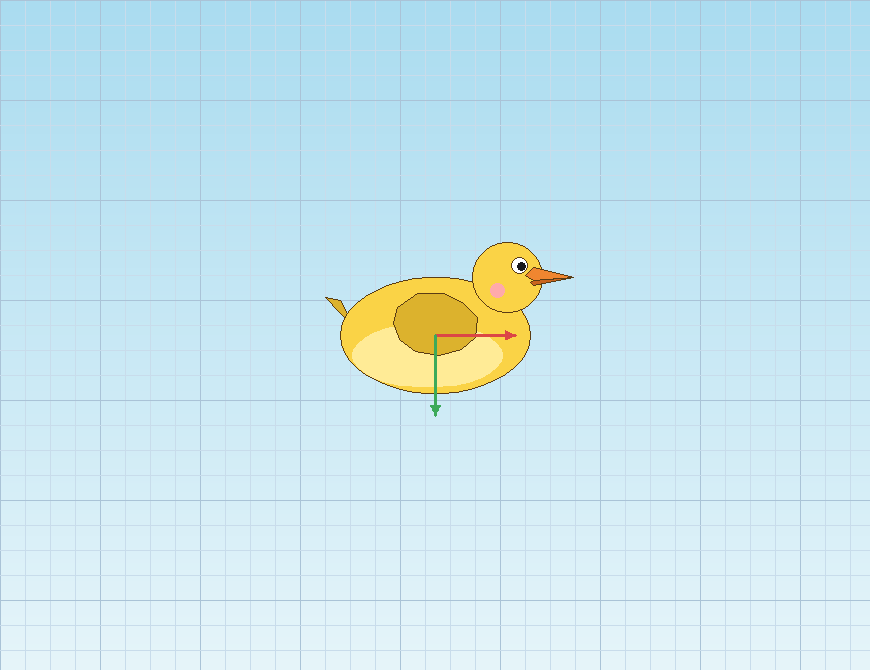
\includegraphics[width=0.5\textwidth]{images/duck_default.png}
\caption{题目二 · 默认姿态}
\label{fig:duck-default}
\end{figure}

\begin{figure}[H]
\centering
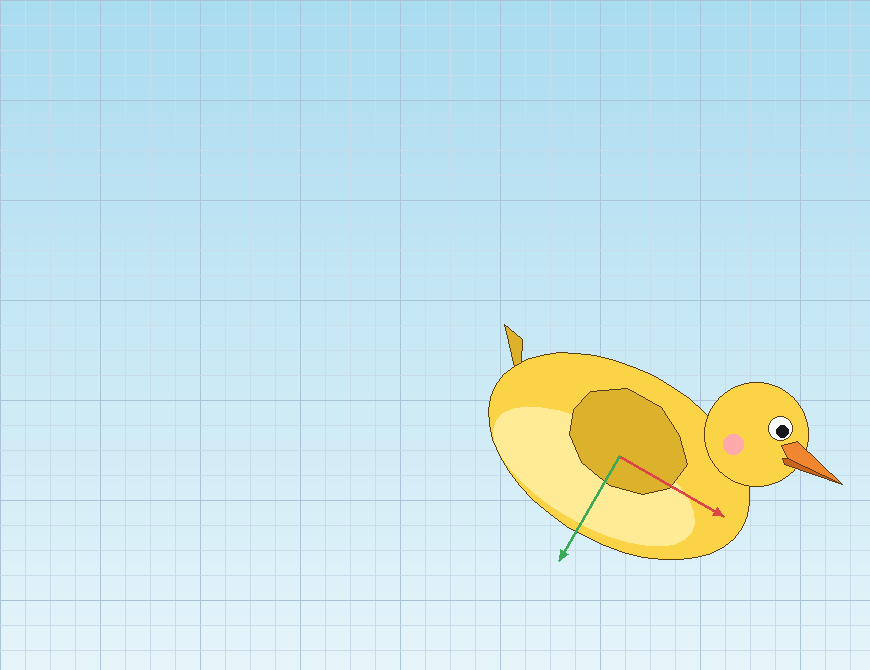
\includegraphics[width=0.5\textwidth]{images/duck_trans.png}
\caption{旋转 30° / 缩放 1.5×/平移的鸭子姿态}
\label{fig:duck-transforms}
\end{figure}


\subsection{题目三：游泳的鸭子}

题目三是任务书指定的\textit{提高题}。在题目二复用的算法栈
（Bresenham 直线、中点画圆、扫描线填充、2D 齐次变换、鸭子模型）之上，
本模块新引入了任务书重点提及的"图形裁剪"——具体实现
\textbf{Sutherland--Hodgman 多边形裁剪算法}，并把它落地到一个
有说服力的可视场景：游泳的鸭子在水线处被切成水上水下两段，
水下子多边形用蓝色调重新填充。

\subsubsection*{4.3.1\quad 算法原理}

\paragraph{（一）Sutherland--Hodgman 多边形裁剪}~

\textbf{问题}：给定一个主多边形 $P$ 和一条裁剪有向直线 $L$，
求 $P$ 落在 $L$ 内侧的那部分子多边形。

\textbf{思想}：依次遍历 $P$ 的每条边 (prev → cur)。
约定"内侧"为 $L$ 的右侧（叉积 $\le 0$ 一侧），将边的两端点对
$L$ 做"内 / 外"判定，得到四种情况：

\begin{table}[H]
\centering
\renewcommand{\arraystretch}{1.3}
\begin{tabular}{|c|c|p{8cm}|}
\hline
prev & cur & 输出到结果多边形 \\
\hline
内 & 内 & 输出 cur \\
\hline
内 & 外 & 输出 (prev, cur) 与 $L$ 的交点 \\
\hline
外 & 内 & 先输出交点，再输出 cur \\
\hline
外 & 外 & 都不输出 \\
\hline
\end{tabular}
\caption{Sutherland--Hodgman 算法的四种边端点情况}
\end{table}

完成一轮遍历后即得到对单条裁剪线裁剪后的子多边形。
对凸的裁剪窗口（如矩形 / 三角形 / 任意凸多边形），只需对每条裁剪边
逐次迭代调用上述过程，前一次的输出作为后一次的输入，
最终得到完整的裁剪结果。

\textbf{内 / 外判定}：用叉积。点 $P = (x, y)$ 对有向直线
$L: P_1(x_1, y_1) \to P_2(x_2, y_2)$ 的有向距离指示量
\[
\mathrm{side}(P) = (x_2 - x_1)(y - y_1) - (y_2 - y_1)(x - x_1).
\]
$\mathrm{side}(P) \le 0$ 表示 $P$ 在 $L$ 右侧（内侧），否则在外侧。

\textbf{交点求解}：直线 $P_1 P_2$ 与线段 $A B$ 的交点用参数法求解。
设交点 $= P_1 + t(P_2 - P_1)$，联立方程：
\[
t = \frac{(x_1 - x_3)(y_3 - y_4) - (y_1 - y_3)(x_3 - x_4)}
        {(x_1 - x_2)(y_3 - y_4) - (y_1 - y_2)(x_3 - x_4)}.
\]

\begin{lstlisting}[language=Python, caption={Sutherland--Hodgman 裁剪（algorithms.py 摘录）}]
def clip_polygon_against_line(polygon, p1, p2):
    if not polygon: return []
    x1, y1 = p1
    x2, y2 = p2

    def side(p):
        return (x2 - x1) * (p[1] - y1) - (y2 - y1) * (p[0] - x1)

    def intersect(a, b):
        x3, y3 = a; x4, y4 = b
        denom = (x1 - x2) * (y3 - y4) - (y1 - y2) * (x3 - x4)
        if abs(denom) < 1e-9: return a
        t = ((x1 - x3) * (y3 - y4) - (y1 - y3) * (x3 - x4)) / denom
        return (x1 + t * (x2 - x1), y1 + t * (y2 - y1))

    result = []
    n = len(polygon)
    for i in range(n):
        cur, prev = polygon[i], polygon[i - 1]
        cur_in  = side(cur)  <= 0
        prev_in = side(prev) <= 0
        if cur_in:
            if not prev_in: result.append(intersect(prev, cur))
            result.append(cur)
        elif prev_in:
            result.append(intersect(prev, cur))
    return result
\end{lstlisting}

针对常用的水平线裁剪，再封装一个便利函数：

\begin{lstlisting}[language=Python, caption={水平线裁剪封装}]
def clip_polygon_horizontal(polygon, y_line, keep="below"):
    # pygame y 向下：方向 +x 时叉积 <= 0 一侧 = 水线上方
    if keep == "below":
        p1, p2 = (1, y_line), (0, y_line)
    else:
        p1, p2 = (0, y_line), (1, y_line)
    return clip_polygon_against_line(polygon, p1, p2)
\end{lstlisting}

\paragraph{（二）游泳动画的物理直觉}~

游泳动画由复合变换 $M = T \cdot R \cdot S$ 的三个分量分别承载三种运动：

\begin{itemize}[leftmargin=*]
    \item \textbf{水平游动} $\Rightarrow$ $T$ 的 $t_x$：每帧
    $t_x \mathrel{+{=}} v \cdot d$，其中 $v$ 是游泳速度、$d \in \{+1, -1\}$ 是方向；
    碰到画布边缘 $d$ 自动取反并把鸭子缩放因子 $s_x = \pm 1$ 翻转，
    保证头朝运动方向。
    \item \textbf{上下浮沉} $\Rightarrow$ $T$ 的 $t_y$：
    $t_y = y_{\text{水线}} - 28 + A_b \sin(\omega t)$，
    $A_b$ 为浮沉幅度。
    \item \textbf{左右摇摆} $\Rightarrow$ $R$ 的旋转角：
    $\theta = A_r \sin(1.3\, \omega t)$。频率略高于浮沉，
    使两种运动节奏交错，看起来更自然。
\end{itemize}

\paragraph{（三）水面正弦扰动}~

水线 $y = y_w$ 用一维正弦扰动表现波动：
\[
y_{\text{波面}}(x) = y_w + A_w \sin(k\,x + \omega_w t),
\]
其中 $A_w \approx 2.5$ 像素、$k = 0.025$ 频率系数。
每帧沿 $x$ 方向逐像素绘制白色细线，并在其上方再画一像素更亮的颜色，
营造水面"细高光"的视觉效果。

\paragraph{（四）涟漪}~

涟漪是\textbf{时变粒子系统}。每个涟漪是一个三元组
$(c_x, c_y, r, t)$：圆心固定，半径 $r$ 每帧增长 $\sim 1.4$ 像素，
年龄 $t$ 计数。用中点画圆算法生成圆周像素，
但\textit{只保留位于水面线附近}（$|y - y_w| \le 2$）的部分，
模拟"水面波纹"而非完整圆。颜色按生命比例线性渐隐：
\[
\mathrm{color}(t) = \mathrm{base} \cdot \left(1 - \frac{t}{t_{\max}}\right).
\]
速度越大涟漪发射频率越高（冷却时间 $= \max(8, 28 - 8v)$ 帧）。

\subsubsection*{4.3.2\quad 主要功能模块设计}

题目三完全复用题目二的 \texttt{transforms.py / duck.py / widgets.py}，
\texttt{algorithms.py} 在原有四种基本算法之外新增两个裁剪函数。
\texttt{main.py} 中实现 \texttt{SwimmingScene} 与 \texttt{App} 两个类。

\begin{figure}[H]
\centering
\fbox{\parbox[c][4.6cm][c]{0.85\textwidth}{\centering
\ttfamily
main.py（App + SwimmingScene）\\
$\downarrow$ 调用 $\downarrow$ \\
duck.py(Duck) $\quad\to\quad$ transforms.py（matrices）\\
$\downarrow$ \\
algorithms.py \\
（Bresenham / 中点圆 / 扫描线填充 / \textbf{Sutherland--Hodgman 裁剪}）
\quad widgets.py（Button / Toggle / Slider）
}}
\caption{题目三模块依赖关系（粗体为新增算法）}
\label{fig:module-swim}
\end{figure}

\texttt{SwimmingScene} 的关键状态：
\begin{itemize}[leftmargin=*]
    \item \texttt{duck\_x, swim\_dir, swim\_speed}\,——鸭子水平位置、方向、速度；
    \item \texttt{bob\_amp, rock\_amp\_deg}\,——浮沉与摇摆幅度；
    \item \texttt{water\_y\_ratio}\,——水线高度（占画布高度比例）；
    \item \texttt{ripples}\,——涟漪粒子列表 \texttt{[\{cx, cy, r, age, max\_age\}, ...]}；
    \item \texttt{theme\_name}\,——三套配色之一（白昼 / 黄昏 / 月夜）；
    \item \texttt{show\_clipping / show\_clip\_debug / show\_ripples}\,——视图开关。
\end{itemize}

\subsubsection*{4.3.3\quad 实现流程}

\paragraph{游泳变换矩阵的组装}\ 三种运动通过 $T \cdot R \cdot S$ 一次性叠加：

\begin{lstlisting}[language=Python, caption={游泳变换组装（main.py 摘录）}]
def _duck_transform(self):
    t = self.frame * 0.05
    bob_y = self.bob_amp * math.sin(t)
    rock  = math.radians(self.rock_amp_deg) * math.sin(t * 1.3)
    sx = -1.0 if self.swim_dir < 0 else 1.0   # 头朝运动方向
    wy = self.water_y
    cy = wy - 28 + bob_y                       # 略高于水面，腹部入水
    return compose(
        translate(self.duck_x, cy),            # 水平游动 + 浮沉
        rotate(rock),                          # 左右摇摆
        scale(sx, 1.0),                        # 镜像翻转
    )
\end{lstlisting}

\paragraph{水下染色 —— 裁剪算法的实战应用}\ 鸭子先按平时的方式完整渲染一次；
然后取出身体和腹部多边形，把世界坐标顶点对水线做 Sutherland--Hodgman 裁剪，
得到水下子多边形，再用扫描线填充以水蓝色覆盖在已渲染的鸭子之上：

\begin{lstlisting}[language=Python, caption={水下染色（main.py 摘录）}]
def _draw_duck(self):
    M = self._duck_transform()
    # 1) 整鸭按常规渲染
    self.duck.render(self.surface, M, self._put)

    # 2) 把身体/腹部多边形裁剪到水线下方，重新填充水色
    if self.show_clipping:
        wy = self.water_y
        uw_color = self.theme["underwater"]
        for part in (self.duck.body, self.duck.belly):
            world_verts = [(int(round(x)), int(round(y)))
                           for x, y in apply_points(M, part)]
            below = clip_polygon_horizontal(world_verts, wy, keep="below")
            below = [(int(round(x)), int(round(y))) for x, y in below]
            if len(below) >= 3:
                self._put(self.surface,
                          scanline_fill_polygon(below), uw_color)
\end{lstlisting}

\paragraph{涟漪的发射、更新与渲染}~

\begin{lstlisting}[language=Python, caption={涟漪粒子系统（main.py 摘录）}]
def _emit_ripple(self):
    bx = int(self.duck_x - 80 * self.swim_dir)
    self.ripples.append({"cx": bx, "cy": self.water_y, "r": 2.0,
                         "age": 0, "max_age": 70})

def _update_ripples(self):
    for rp in self.ripples:
        rp["r"]   += 1.4
        rp["age"] += 1
    self.ripples = [r for r in self.ripples if r["age"] < r["max_age"]]

def _draw_ripples(self):
    wy = self.water_y
    base = self.theme["ripple"]
    for rp in self.ripples:
        alpha = 1.0 - rp["age"] / rp["max_age"]
        c = tuple(int(b * alpha) for b in base)
        pts = midpoint_circle(rp["cx"], rp["cy"], int(rp["r"]))
        for x, y in pts:
            if abs(y - wy) <= 2:           # 只保留水面附近的圆弧
                if 0 <= x < self.w and 0 <= y < self.h:
                    self.surface.set_at((x, y), c)
\end{lstlisting}

\paragraph{自动游泳与边界反弹}~

\begin{lstlisting}[language=Python, caption={步进逻辑（main.py 摘录）}]
def _step(self):
    if self.paused or self.dragging:
        return
    self.frame += 1
    self.duck_x += self.swim_speed * self.swim_dir
    margin = 100
    if self.duck_x < margin:
        self.duck_x = margin; self.swim_dir = 1
    elif self.duck_x > self.w - margin:
        self.duck_x = self.w - margin; self.swim_dir = -1
    self.ripple_cd -= 1
    if self.ripple_cd <= 0:
        self._emit_ripple()
        self.ripple_cd = max(8, int(28 - self.swim_speed * 8))
    self._update_ripples()
\end{lstlisting}

\paragraph{裁剪调试可视化}\ 开启"裁剪调试"开关后：
\begin{itemize}[leftmargin=*]
    \item 在画布上叠加水线（红色横线）；
    \item 给裁剪后的水下子多边形描黄色边框（Bresenham 直线）；
    \item 在 $|y - y_w| \le 1$ 的裁剪交点位置画一个红色小圆点。
\end{itemize}
这让 Sutherland--Hodgman 算法的输出可以\textit{直接被肉眼验证}——
能看到交点正好落在水线上、子多边形与水线无缝相接。

\subsubsection*{4.3.4\quad 运行效果}

\begin{figure}[H]
\centering
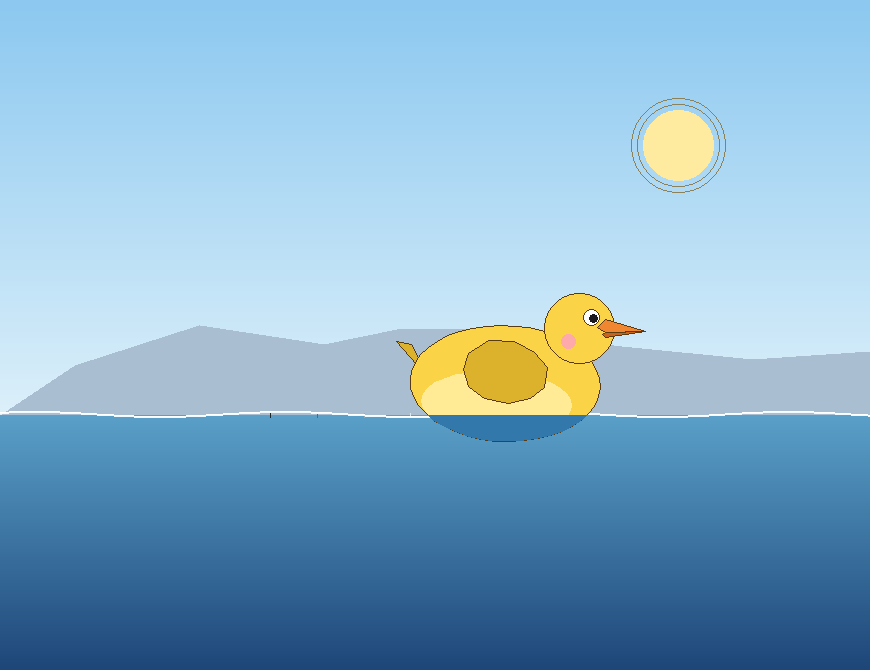
\includegraphics[width=0.5\textwidth]{images/swim_duck_000.png}
\caption{题目三 · 游泳的鸭子（白昼）}
\label{fig:swim-main}
\end{figure}


\begin{figure}[H]
\centering
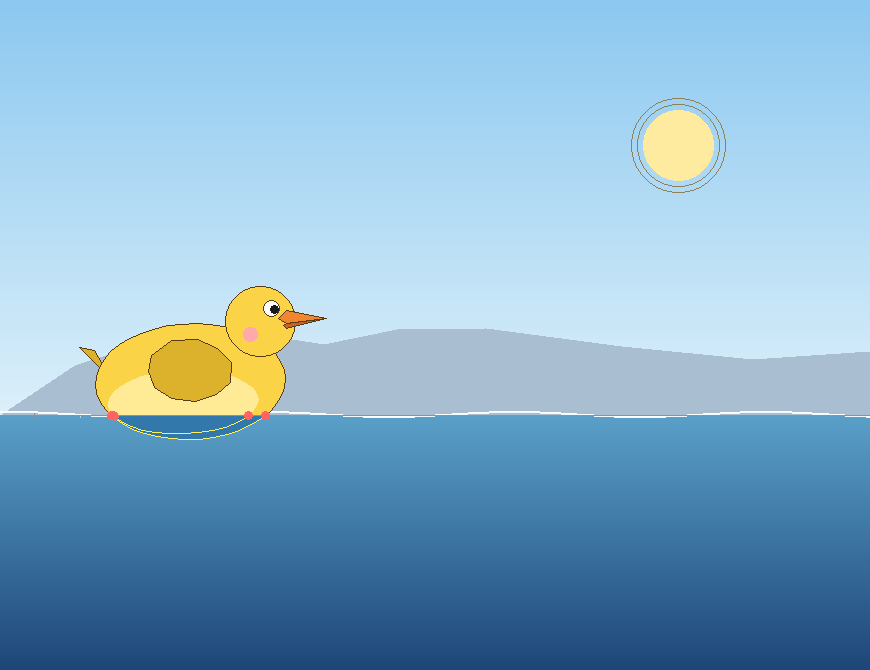
\includegraphics[width=0.5\textwidth]{images/swim_duck_001.png}
\caption{Sutherland--Hodgman 裁剪可视化（调试模式）}
\label{fig:swim-clip-debug}
\end{figure}

\subsection{题目四：松树与松果}

题目四是任务书指定的\textit{难题}。本模块是整个课程设计的"算法集大成者"——
直接复用前三题的算法库，新引入\textbf{De Casteljau Bezier 曲线}
作为关键图形学算法，并以\textbf{基于矩阵的层级化变换}与
\textbf{简单刚体物理}两套机制驱动整个场景的动画。

\subsubsection*{4.4.1\quad 算法原理}

\paragraph{（一）De Casteljau 算法与 Bezier 曲线}~

$n$ 阶 Bezier 曲线由 $n+1$ 个控制点 $P_0, P_1, \ldots, P_n$ 定义，
参数形式为
\[
B(t) = \sum_{i=0}^{n} \binom{n}{i} (1-t)^{n-i} t^i P_i,
\qquad t \in [0, 1].
\]
直接代入二项展开计算\textit{数值稳定性差}，且每阶需要重新推导。
\textbf{De Casteljau 算法}给出了一种\textit{递推式}求值方法，
只用\textit{反复的线性插值}：

\begin{align*}
P_i^{(0)} &= P_i,\qquad i = 0, 1, \ldots, n,\\
P_i^{(k)} &= (1 - t)\, P_i^{(k-1)} + t\, P_{i+1}^{(k-1)},
\qquad k = 1, \ldots, n,
\end{align*}
最终 $P_0^{(n)}$ 即为曲线上参数 $t$ 处的点。每一轮把控制点数减少 1，
经过 $n$ 轮（$O(n^2)$ 次插值）即可得到结果。
该算法\textbf{数值稳定}、\textbf{几何直观}（每轮的中间点连成的折线
逐渐"塌缩"到曲线上一点），并可推广到任意阶。

\begin{lstlisting}[language=Python, caption={De Casteljau 算法（algorithms.py 摘录）}]
def de_casteljau(control_points, t):
    pts = [(float(x), float(y)) for x, y in control_points]
    while len(pts) > 1:
        nxt = []
        for i in range(len(pts) - 1):
            x = (1 - t) * pts[i][0] + t * pts[i + 1][0]
            y = (1 - t) * pts[i][1] + t * pts[i + 1][1]
            nxt.append((x, y))
        pts = nxt
    return pts[0]

def bezier_curve(control_points, segments=24):
    return [de_casteljau(control_points, i / segments) for i in range(segments + 1)]
\end{lstlisting}

\paragraph{（二）Bezier 曲线在松树枝叶中的应用}~

每层 tier 的下垂底边用一条\textbf{二次 Bezier}生成：
控制点取
\[
P_0 = (-w, y_{\text{底}}),\quad
P_1 = (0,\, y_{\text{底}} + 0.4\, h),\quad
P_2 = (w,\, y_{\text{底}}),
\]
其中 $w$ 为该层半宽、$h$ 为该层高度。$P_1$ 位于两端点下方
（pygame y 向下，$y_{\text{底}} + 0.4h$ 比端点更靠下），
故曲线\textit{向下凸}，给枝叶一种自然垂坠感。
采样 18 段后与左右斜边及顶点拼成 20 顶点多边形，
直接送入扫描线填充。

\paragraph{（三）基于矩阵的层级化摇摆}~

设树根在世界位置 $(x_0, y_0)$，则\textit{树→世界}的基变换为
$M_{\text{base}} = T(x_0, y_0)$。
每层 tier 在树坐标系中以自身底边 $(0, y_i)$ 为支点旋转，
旋转矩阵为
\[
M_{\text{sway},i} = T(0, y_i) \cdot R(\theta_i) \cdot T(0, -y_i),
\]
其中摆动角度按高度递增：
\[
\theta_i = A_i \cdot w_{\text{wind}} \cdot \sin(\omega t + \varphi_i),
\qquad
A_i = A_{\min} + (A_{\max} - A_{\min}) \cdot \frac{i}{N - 1}.
\]
最终每层的\textit{世界变换}由树基变换与自身摇摆复合：
\[
M_{\text{world},i} = M_{\text{base}} \cdot M_{\text{sway},i}.
\]
这与角色骨骼动画中"父骨头矩阵 $\cdot$ 子骨头局部矩阵"的原理一致，
是\textbf{层级化变换}（hierarchical transformation）的最简实现。

枝头位置——也即松果挂载点——同样位于 tier 局部坐标中（底边的 4 个采样点之一），
经 $M_{\text{world},i}$ 变换即得每帧的世界位置，
让\textit{挂着的松果自然随着枝叶一起摇晃}。

\paragraph{（四）松果的物理仿真}~

每颗松果维护一个三状态机：

\begin{table}[H]
\centering
\renewcommand{\arraystretch}{1.3}
\begin{tabular}{|c|p{4.4cm}|p{6cm}|}
\hline
\textbf{状态} & \textbf{位置来源} & \textbf{转换条件} \\
\hline
ATTACHED & 每帧同步对应枝头世界位置 &
\textit{摇晃}按钮 / 自动倒计时 / 鼠标点击附近 \\
\hline
FALLING & 物理积分（重力 + 风 + 阻力） & $y \ge y_{\text{地面}}$ 时落地 \\
\hline
LANDED & 停在落地位置 & 无（直至重置） \\
\hline
\end{tabular}
\caption{松果状态机}
\end{table}

物理积分（每帧 $\Delta t = 1$）：
\[
v_y \mathrel{+{=}} g,\quad
v_x \mathrel{+{=}} w_{\text{wind}} \cdot k_w,\quad
\begin{aligned}v_x \mathrel{*{=}} d \\ v_y \mathrel{*{=}} d\end{aligned},\quad
x \mathrel{+{=}} v_x,\;
y \mathrel{+{=}} v_y,\;
\theta \mathrel{+{=}} v_a,
\]
其中 $g = 0.35$ 为重力加速度、$k_w = 0.05$ 为风力耦合系数、
$d = 0.992$ 为空气阻力。脱落瞬间给定一个小的随机初速 $(v_x, v_y, v_a)$，
模拟松果"被颠下来"的不规则运动。

\subsubsection*{4.4.2\quad 主要功能模块设计}

题目四进一步丰富了通用算法库，并新增两个领域模块：

\begin{itemize}[leftmargin=*]
    \item \texttt{algorithms.py}\,——在原有四种算法基础上新增
    \texttt{de\_casteljau} 与 \texttt{bezier\_curve} 两个函数。
    \item \texttt{tree.py}\,——新增。\texttt{TreeTier} 封装一层枝叶
    （Bezier 底边 + 摇摆矩阵），\texttt{PineTree} 管理树干与多层 tier，
    提供 \texttt{render} 与 \texttt{branch\_tip\_world\_positions} 接口。
    \item \texttt{pinecone.py}\,——新增。\texttt{Pinecone} 实现三状态机、
    物理积分和外观渲染（橄榄形多边形 + 6 条 Bresenham 鳞片纹理）。
    \item \texttt{transforms.py / widgets.py}\,——直接复用，零修改。
    \item \texttt{main.py}\,——\texttt{ForestScene}（场景管理、参数控制、
    主题、松果调度）+ \texttt{App}（窗口 + UI + 事件循环）。
\end{itemize}

\begin{figure}[H]
\centering
\fbox{\parbox[c][5.2cm][c]{0.85\textwidth}{\centering
\ttfamily
main.py（App + ForestScene）\\
$\downarrow$ \\
tree.py（PineTree, TreeTier）$\quad$
pinecone.py（Pinecone：三状态机 + 物理）\\
$\downarrow$ \\
transforms.py（matrices）\\
$\downarrow$ \\
algorithms.py（Bresenham / 中点圆 / 扫描线 / \textbf{Bezier} / 裁剪）
\quad widgets.py
}}
\caption{题目四模块依赖关系（粗体为本题新增算法）}
\label{fig:module-tree}
\end{figure}

\subsubsection*{4.4.3\quad 实现流程}

\paragraph{Bezier 曲线生成枝叶轮廓}~

\begin{lstlisting}[language=Python, caption={tier 静态轮廓（tree.py 摘录）}]
class TreeTier:
    def __init__(self, base_y, half_width, height, ...):
        self.base_y, self.w, self.h = base_y, half_width, height
        # 底边：二次 Bezier，控制点 P1 在 (0, base_y + 0.4h)
        bottom = bezier_curve(
            [(-self.w, self.base_y),
             ( 0.0,    self.base_y + 0.4 * self.h),
             ( self.w, self.base_y)],
            segments=18,
        )
        apex = (0.0, self.base_y - self.h)
        self.local_polygon = bottom + [apex]    # 19 + 1 = 20 顶点
        # 枝头：从底边采样里挑 4 个点作为松果挂载位置
        n = len(bottom)
        self.branch_tips_local = [bottom[i] for i in
                                  (int(n*0.15), int(n*0.4),
                                   int(n*0.6),  int(n*0.85))]
\end{lstlisting}

\paragraph{tier 摇摆矩阵与世界变换}~

\begin{lstlisting}[language=Python, caption={层级化变换（tree.py 摘录）}]
def tier_world_matrices(self, base_M, t, wind_strength=1.0):
    """[(tier, M_world), ...] 每层叠加自身摇摆 + 父变换"""
    result = []
    for tier in self.tiers:
        theta = (math.radians(tier.sway_amp_deg) * wind_strength
                 * math.sin(t + tier.sway_phase))
        M_sway = compose(translate(0, tier.base_y),
                         rotate(theta),
                         translate(0, -tier.base_y))
        result.append((tier, compose(base_M, M_sway)))   # 父 ⋅ 子
    return result
\end{lstlisting}

\paragraph{松果挂载位置同步}\ 每帧 \texttt{ForestScene} 都要把所有
ATTACHED 状态的松果的世界位置同步到当前枝头位置（枝头本身因
摇摆而移动）：

\begin{lstlisting}[language=Python, caption={松果挂载同步（main.py 摘录）}]
tips = self.tree.branch_tip_world_positions(base_M, t, wind_strength=1.0)
tips_map = {(ti, ki): pos for ti, ki, pos in tips}
for pc in self.pinecones:
    if pc.state == Pinecone.STATE_ATTACHED:
        pos = tips_map.get((pc.tier_idx, pc.tip_idx))
        if pos is not None:
            pc.attach_to(pos)
    else:
        pc.step(self.wind, self.ground_y - 2)
\end{lstlisting}

\paragraph{松果物理积分}~

\begin{lstlisting}[language=Python, caption={物理 step（pinecone.py 摘录）}]
def step(self, wind_x, ground_y):
    if self.state != self.STATE_FALLING:
        return
    self.vy += GRAVITY                  # 重力
    self.vx += wind_x * WIND_COEF       # 风力
    self.vx *= DRAG                     # 空气阻力
    self.vy *= DRAG
    self.x  += self.vx
    self.y  += self.vy
    self.angle += self.va               # 自旋
    if self.y >= ground_y:              # 落地
        self.y = ground_y
        self.state = self.STATE_LANDED
        self.vx = self.vy = self.va = 0.0
\end{lstlisting}

\paragraph{Bezier 控制点的可视化}\ 开启"Bezier 控制点显示"开关后，
底层 tier 的 3 个控制点（红色实心圆）和它们的控制多边形（粉色折线）
被画在画布上。控制点会跟随该层 tier 的摇摆一起旋转，
让"曲线的几何意义"\textit{动起来}：观察者可以直观感受
"控制多边形向曲线靠近"这一 De Casteljau 的核心几何性质。

\subsubsection*{4.4.4\quad 运行效果}

\begin{figure}[H]
\centering

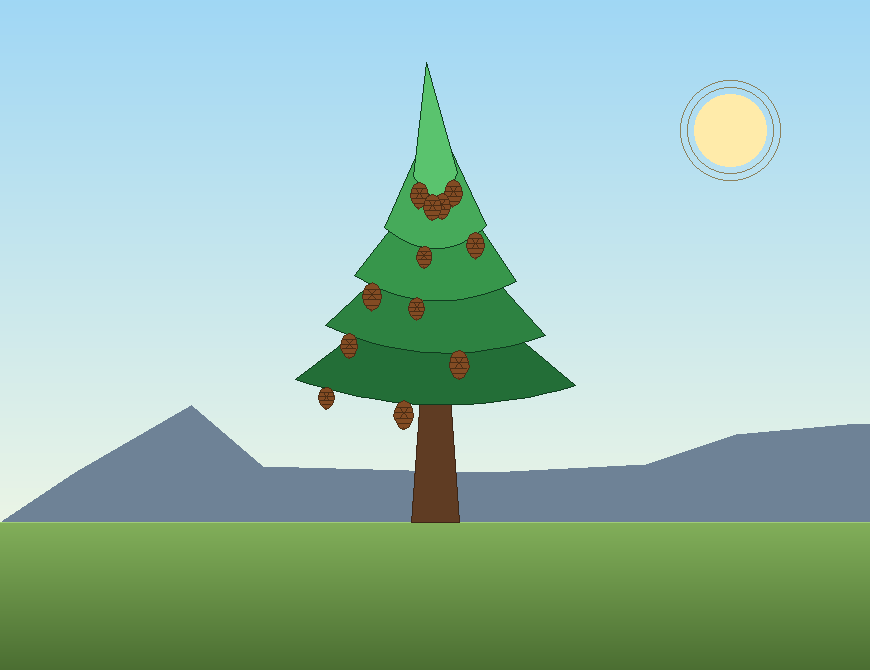
\includegraphics[width=0.5\textwidth]{images/pinetree_000.png}
\caption{题目四 · 默认状态（春日）}
\label{fig:tree-main}
\end{figure}

\begin{figure}[H]
\centering
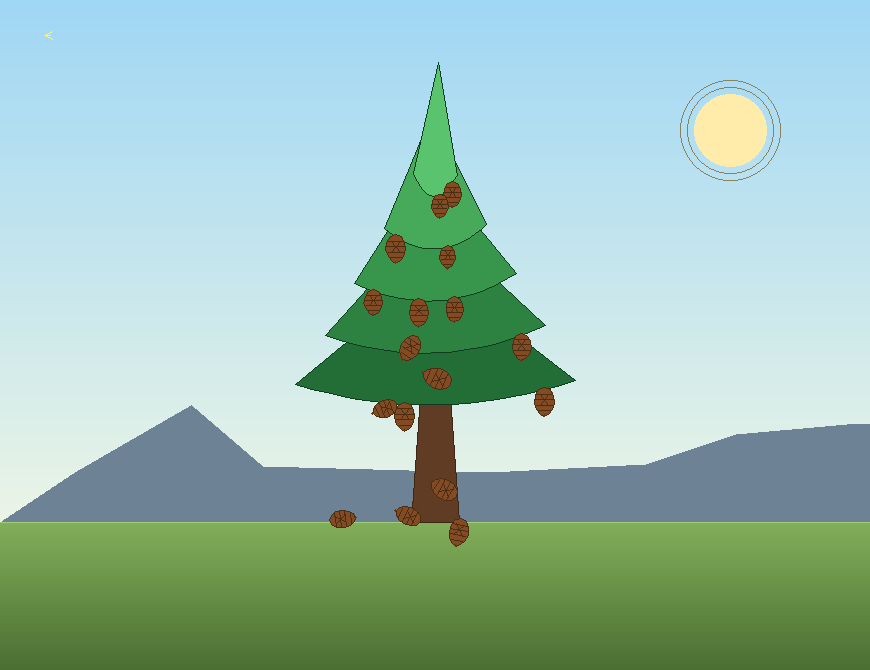
\includegraphics[width=0.5\textwidth]{images/pinetree_001.png}
\caption{物理仿真：风力 + 重力 + 自旋的松果掉落}
\label{fig:tree-fall}
\end{figure}

\begin{figure}[H]
\centering

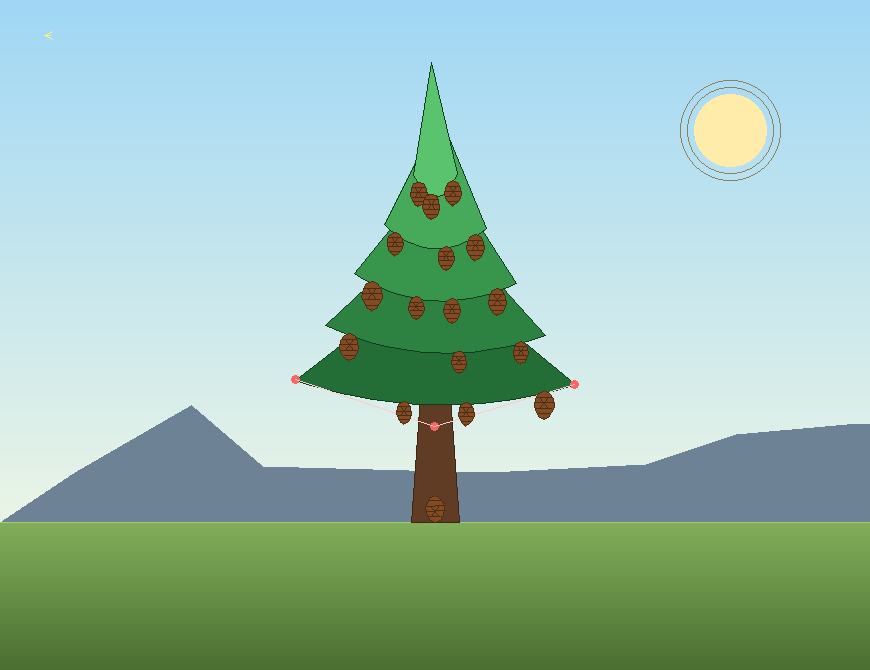
\includegraphics[width=0.5\textwidth]{images/pinetree_002.png}
\caption{De Casteljau Bezier 控制点的几何可视化}
\label{fig:tree-bezier}
\end{figure}


% --------- 五、总结 ---------
\section{总结}\label{sec:five}

\subsection{程序结构优缺点分析}

\paragraph{优点}~

\begin{itemize}[leftmargin=*]
    \item \textbf{算法与渲染解耦}：\texttt{algorithms.py} 是纯函数库，输入几何参数、
    输出像素坐标，不依赖 \texttt{pygame.Surface} 或任何渲染上下文。
    这样既便于单元测试，也允许该模块直接在题目二/三/四中复用，无需任何改动。
    % 
    $7\times 10^5$ 降到约 $1.5\times 10^4$，使得在普通笔记本上也能流畅运行。
    \item \textbf{交互完整}：菜单栏（按钮 + 开关）、参数面板（滑块）、快捷键、
    保存图片、关于弹窗一应俱全，满足任务书"界面美观、衔接自然、注重交互性"的要求。
\end{itemize}

\paragraph{缺点与改进方向}~

\begin{itemize}[leftmargin=*]

    \item \textbf{扫描线填充未做边表加速}：教科书做法是\textbf{活动边表}（AET），
    扫描线推进时增量维护边表，复杂度从 $O(\text{边数} \times \text{扫描线数})$
    降到 $O(\text{像素数})$。本实现采用最朴素的"逐扫描线遍历所有边"，
    凹多边形顶点不多时差异不显著，但对复杂图形仍有优化空间。

\end{itemize}

\subsection{出错原因分析}

开发过程中遇到的主要问题及解决：

\begin{enumerate}[label=（\arabic*）, leftmargin=*]
    \item \textbf{Pygame 字体初始化崩溃}\quad
    第一次启动时报错
    \texttt{TypeError: expected str, bytes or os.PathLike object, not int}，
    来自 \texttt{pygame.font.sysfont.initsysfonts\_win32}。
    原因是本机 Windows 字体注册表中存在\textit{非字符串类型}的项
    （某些被损坏的字体条目），\texttt{splitext} 期望字符串而拿到整数。
    \textbf{解决}：彻底跳过 \texttt{pygame.font.SysFont} 与
    \texttt{pygame.font.get\_fonts}，改为通过
    \texttt{pygame.font.Font(r"C:\textbackslash{}Windows\textbackslash{}Fonts\textbackslash{}msyh.ttc", size)}
    \textit{按文件路径}加载字体，绕开有问题的系统字体扫描过程。

    \item \textbf{扫描线在顶点处的"漏填"或"过填"}\quad
    最初版本在多边形顶点处偶尔出现单像素瑕疵。
    原因是当扫描线 $y$ 恰好等于某个顶点 $y_0$ 时，
    若该顶点被两条边同时计入，会得到\textit{奇数个交点}，配对失败。
    \textbf{解决}：约定每条边\textit{包含下端点而不含上端点}（条件 $y_0 \le y < y_1$），
    顶点只会被位于其下方的那条边计入一次。

    \item \textbf{中文字符显示成方块}\quad
    最初使用 \texttt{pygame.font.Font(None, ...)} 加载默认字体，
    所有中文显示为方块（\texttt{tofu}）。
    \textbf{解决}：定位到 \texttt{msyh.ttc / simhei.ttf} 等系统中文字体文件后按路径加载。

    \item \textbf{逐帧重画整个场景导致掉帧}\quad
    初版每帧都重画渐变背景（720 行扫描）+ 山脉填充（$\sim$50000 像素）+
    月亮填充（$\sim$8000 像素），帧率约 12\,FPS。
    \textbf{解决}：把这三者画到一张缓存 Surface 上，每帧只 \texttt{blit} 复用，
    仅动态元素重画，稳定 60\,FPS。

    \item \textbf{彗星拖尾不够"软"}\quad
    最初拖尾使用等亮度直线，视觉突兀。
    \textbf{解决}：沿尾巴方向按距离平方衰减
    $\alpha = (1 - i/L)^{1.5}$，让尾巴远端自然过渡到背景。

    \item \textbf{Sutherland--Hodgman 裁剪方向反了}\quad
    题目三实现 \texttt{clip\_polygon\_horizontal(poly, y, keep="below")}
    后单元测试发现：用三角形 $(0,0)\text{-}(10,0)\text{-}(5,10)$、$y_{\text{线}}=5$
    时，\texttt{keep="below"} 竟然返回了\textit{上半}（含 $(0,0)$ 与 $(10,0)$）。
    原因：算法约定"内侧"为有向直线\textbf{右侧}（叉积 $\le 0$），
    而 pygame 中 $y$ 向下——一条沿 $+x$ 方向的水平线，其右侧
    （叉积 $\le 0$）对应 $y \le y_{\text{线}}$，正是水线\textit{上方}。
    \textbf{解决}：把 \texttt{keep="below"} 对应的有向直线
    取反方向（$p_1, p_2 = (1, y), (0, y)$），让 $-x$ 方向直线的
    右侧（叉积 $\le 0$）对应 $y \ge y_{\text{线}}$，与"水下"含义一致。
    教训：坐标系朝向（$y$-up vs.\ $y$-down）必须事先核对，
    几何算法的方向约定要用单元测试单独验证，不能依赖肉眼调 UI。

    \item \textbf{涟漪用完整圆显得不自然}\quad
    最初把涟漪当作正圆全部画出来，俯视感太强，与侧面游泳视角冲突。
    \textbf{解决}：仍用中点画圆生成全圆像素，但渲染时只保留满足
    $|y - y_w| \le 2$ 的部分，得到"水面带状波纹"效果，
    符合人在水边平视所看到的水波形态。

    \item \textbf{Bezier 采样段数的精度/性能权衡}\quad
    题目四的 tier 底边 Bezier 一开始采样 8 段，曲线在中段呈现可见的折线感，
    破坏"枝叶下垂"的圆润视觉。提到 36 段后又显著影响每帧的扫描线填充耗时
    （多边形顶点更多 → 边表更长）。\textbf{解决}：折中取 18 段，
    肉眼几乎察觉不到折角，扫描线填充的额外开销可以忽略。
    更一般的做法是\textbf{自适应分段}（根据曲线曲率细分），
    但本作品的曲线很短小，固定段数已经足够。

    \item \textbf{层级摇摆放大失控}\quad
    题目四最初尝试做"完整层级"——每层 tier 的旋转矩阵叠加在
    \textit{上一层}已变换的世界矩阵之上（$M_i = M_{i-1} \cdot M_{\text{sway},i}$），
    模拟"枝叶根部跟着上一层底部一起摇"。实际上这种连乘\textit{角度累积过快}：
    顶层有效摆动可达 $20^\circ$ 以上，看起来更像柳枝、不像松树。
    \textbf{解决}：改为"父变换 + 自身摇摆"两级结构
    （$M_i = M_{\text{base}} \cdot M_{\text{sway},i}$）——
    每层独立绕\textit{自己}的底边摇摆，幅度沿高度\textit{线性}增加而不再连乘，
    动作克制、符合松树韧性强的形象。

    \item \textbf{挂着松果"瞬移"感}\quad
    最初把松果当成独立物体，每帧用 \texttt{attach\_to(world\_xy)} 覆盖位置；
    遇到大风时枝头瞬时变化大，松果显得不连续。
    \textbf{解决}：根本原因不是同步逻辑出错，而是\textit{帧率不稳}让插值断层。
    通过把静态背景（天空 + 远山 + 地面 + 太阳 + 月亮）缓存为一张 Surface，
    每帧只重绘动态部分，帧率回到稳定 60\,FPS，问题消失。
    教训：\textit{表象问题先排查帧率，再怀疑逻辑}。
\end{enumerate}

\end{document}



